%%
%% This is file `sample-authordraft.tex',
%% generated with the docstrip utility.
%%
%% The original source files were:
%%
%% samples.dtx  (with options: `authordraft')
%% 
%% IMPORTANT NOTICE:
%% 
%% For the copyright see the source file.
%% 
%% Any modified versions of this file must be renamed
%% with new filenames distinct from sample-authordraft.tex.
%% 
%% For distribution of the original source see the terms
%% for copying and modification in the file samples.dtx.
%% 
%% This generated file may be distributed as long as the
%% original source files, as listed above, are part of the
%% same distribution. (The sources need not necessarily be
%% in the same archive or directory.)
%%
%% The first command in your LaTeX source must be the \documentclass command.
\documentclass[sigconf]{acmart}
\usepackage{subcaption}
\settopmatter{printacmref=false}
\settopmatter{printacmref=false} % Removes citation information below abstract
\renewcommand\footnotetextcopyrightpermission[1]{} % removes footnote with conference information in first column
\pagestyle{plain} % removes running headers
\usepackage{etoolbox}
\makeatletter
\patchcmd{\maketitle}{\@copyrightpermission}{}{}{}
\makeatother
\usepackage{adjustbox,lipsum}
%%
%% \BibTeX command to typeset BibTeX logo in the docs
\AtBeginDocument{%
  \providecommand\BibTeX{{%
    \normalfont B\kern-0.5em{\scshape i\kern-0.25em b}\kern-0.8em\TeX}}}

%% Rights management information.  This information is sent to you
%% when you complete the rights form.  These commands have SAMPLE
%% values in them; it is your responsibility as an author to replace
%% the commands and values with those provided to you when you
%% complete the rights form.


%% These commands are for a PROCEEDINGS abstract or paper.
% \acmConference[Woodstock '18]{Woodstock '18: ACM Symposium on Neural
%   Gaze Detection}{June 03--05, 2018}{Woodstock, NY}
% \acmBooktitle{Woodstock '18: ACM Symposium on Neural Gaze Detection,
%   June 03--05, 2018, Woodstock, NY}
% \acmPrice{15.00}
% \acmISBN{978-1-4503-9999-9/18/06}


%%
%% Submission ID.
%% Use this when submitting an article to a sponsored event. You'll
%% receive a unique submission ID from the organizers
%% of the event, and this ID should be used as the parameter to this command.
%%\acmSubmissionID{123-A56-BU3}

%%
%% The majority of ACM publications use numbered citations and
%% references.  The command \citestyle{authoryear} switches to the
%% "author year" style.
%%
%% If you are preparing content for an event
%% sponsored by ACM SIGGRAPH, you must use the "author year" style of
%% citations and references.
%% Uncommenting
%% the next command will enable that style.
%%\citestyle{acmauthoryear}

%%
%% end of the preamble, start of the body of the document source.
\begin{document}
\pagestyle{plain}
%%
%% The "title" command has an optional parameter,
%% allowing the author to define a "short title" to be used in page headers.
\title{On-Demand Kinesthetic Guidance for the Visually Impaired}

%%
%% The "author" command and its associated commands are used to define
%% the authors and their affiliations.
%% Of note is the shared affiliation of the first two authors, and the
%% "authornote" and "authornotemark" commands
%% used to denote shared contribution to the research.
\author{Junior Sundar}
\email{Junior.Sundar@colorado.edu}
\affiliation{CSCI 7000}
\affiliation{%
  \institution{University of Colorado Boulder}
  \city{Boulder}
  \state{Colorado}
}

\author{Tenzin Choedon}
\email{Tenzin.Choedon@colorado.edu}
\affiliation{CSCI 7000}
\affiliation{%
  \institution{University of Colorado Boulder}
  \city{Boulder}
  \country{Colorado}}


%%
%% By default, the full list of authors will be used in the page
%% headers. Often, this list is too long, and will overlap
%% other information printed in the page headers. This command allows
%% the author to define a more concise list
%% of authors' names for this purpose.
\renewcommand{\shortauthors}{Sundar and Choedon}

%%
%% The abstract is a short summary of the work to be presented in the
%% article.
\begin{abstract}
Kinesthetic guidance for the visually impaired is a highly relevant research area in human robot interaction. We proposed two methods of kinesthetic guidance, continuous and on-demand. Continuous kinesthetic guidance will guide a person through obstacles from start to end goal by having the person hold on robot arm while on-demand will allow person to navigate to end-goal freely and give feedback when they enter the obstacle region. We are using a Sawyer arm as our guiding agent and setting up our experiment in a Gazebo simulation environment. We are measuring our result by the time it took to get from start to end-goal and the number of collisions for both methods. Our experiment introduces complexity by adding a human arm in the path planning algorithm for an environment with obstacles. 
\end{abstract}

%%
%% The code below is generated by the tool at http://dl.acm.org/ccs.cfm.
%% Please copy and paste the code instead of the example below.
%%

%%
%% Keywords. The author(s) should pick words that accurately describe
%% the work being presented. Separate the keywords with commas.
%\keywords{Cooking recipe; Recipe parsing; Classification; Recipe vectors}

%%
%% This command processes the author and affiliation and title
%% information and builds the first part of the formatted document.
\maketitle
% Introduction
\section{Introduction}
% introduce the problem (explain the motivation: What is it? why solve it?)
% talk about on-demand vs continuous and kinesthetic vs audio guidance
% Hypothesis: What we are testing and what our expected outcome will be
% what we did, breif summary (what you should expect in the report)
There are millions of visually impaired people who are left to depend on other people for help or their guide dog and other resources. To help the visually impaired, in human robot interaction research area, many people have done research in kinesthetic guidance and many more are doing research to improve it to guide a visually impaired person through an obstacle populated environment. Most of the research aims to help a person through the environment from start to end goal. This does not give them independence. There are tools that people are using to help them through like walking stick. Methods researched so far are replacing the walking stick or guide dog. But we believe that the technology should be a tool that will give the person with visually impaired ability to navigate through environment independently as much as possible. Audio guidance could be one of the solution, but it is in the process of development. Therefore, we are proposing two methods of kinesthetic guidance in a controlled environment, which is a table with obstacles placed in different places in our case. In first method, we provide continuous guidance that will allow a person to hold on robot's hand and guide them from start to end goal. In second method, we provide on-demand guidance that will let a person to navigate in our environment independently and interfere when a person's arm enters a collision zone. Participant will experiment both methods and will fill form that will indicate which methods they prefer. We hypothesized that our participant will prefer on-demand guidance over continuous guidance.

Our contribution to the human robot interaction is by adding human arm cost in the environment in kinesthetic guidance. 
So far, most methods calculate cost and navigation path by considering robot's arm as the only agent in the environment. 
In our continuous guidance, we do similar thing. 
We assume human arm will follow same path as robot by holding onto robot's arm. 
In on-demand guidance, human arm is moving independently until it enters collision zone. When human arm enters collision zone, robot arm will enter into the space and help human arm out of collision zone to the goal. 
Now we have two agents in the environment. This add complication. We discuss that in details in Methods section. 

The application domain of our algorithm is as follows. 
Consider a visually-impaired person, searching for an object in a familiar space, but with obstacles whose positions are initially unknown. 
While the individual is confident in moving through this space, they will require intermittent assistance to avoid collisions with obstacles. 
In this situation, we predict that the individual will not require continuous `hand-holding' help and would prefer a greater degree of freedom, while infrequently falling back to assistance from a third-party. 
In our case, we are limiting the workspace to two-dimensions, and expect to extend it to three-dimensions in future works. 
% Related work
\section{Related Work}
Based on a review of published literature, the effectiveness of the variance in kinesthetic guidance has not been fully explored. 
However, there have been some publications looking into the efficacy of audio and vibrotactile feedback modalities. 
In paper \cite{PLosONE}, a study was conducted on the efficiency of implementing vibrotactile and audio feedback systems, and comparing performance to using the cane only. 
It was found that participants could complete a navigation task faster with the the additional feedback systems. 
Comparison between the two systems showed that the participants had faster response and speed with audio feedback as opposed to vibrotactile feedback. 

However, another paper (\cite{IEEE}) which compared the accuracy of performance between audio and vibrotactile feedback systems showed that although the speed of response was faster with audio systems, the accuracy and closeness to a prescribed path was better with haptic feedback. 
Although our project is not trying to approach this problem through a vibrotactile guidance system, this gives us an indication that humans are responsive to tactile guidance. 
This is also supported by the findings of \cite{autonavigation}, where the participants felt vibro-tactile feedback is important and effective. 
In this study, some of the participants thought environment noise could interfere with audio feedback, and thus were not comfortable with this style of feedback. 

Audio feedback guidance has been used frequently. 
Although it is easier to get acquaintances and learn, it does not serve people with low vision. 
Most of the tools have been aimed to serve complete visual impairments and low vision community is widely ignored. People with low vision have some capabilities to see and with the right tools, it can help them guide. 
\cite{smartglasses} designed two wayfinding guidance, audio and visual. 
Visual wayfinding guidance gives an indoor GPS like a route where actions and distance are displayed on the side of the path like a street sign while audio does a similar task through audio feedback. 
Visual wayfinding guidance results were much better than audio but all participants wanted a combination tools of visual and audio that will optimize their wayfinding experience. 
Because both were helpful in different parts of the task.  

The publication in \cite{kinestheticteaching} conducted experiments which were a direct opposite to the goals of our project. 
Their focus was on determining which was the preferred method of teaching a robot to perform a task: through kinesthetic or through teleoperation. 
However, our focus is for the robot to guide the visually-impaired user. 
They found that people prefer kinesthetic over teleoperation due to the learning curve to perform and get comfortable with teleoperation. 
The paper in \cite{humanteacher} did a similar task in teaching robot arm motion to catch a ball. 
They also provided more details about the tools they used to complete and implement their experiment. 

In \cite{robotassist}, the authors compared voice-only assistive robot and collaborative assistive robot for undertaking a task completion. 
Their findings, based on study conducted on 12 blind participants, suggested that people prefer collaborative assistance over voice only assistance.
In their study, they concluded that collaborative assistance was more effective, less time consuming, easier to work with and was socially more acceptable. 
Furthermore, some of the participants had difficulty understanding the commands from voice-only assistive robots. 
% methods
\section{Methods}
The current problem has two components that must be addressed. 
The first requirement is to device a motion planner that can guide the human hand while considering potential collisions of the entire arm with obstacles in the workspace. 
The second requirement is to have a `natural' strategy to interrupt human hand motion, by considering potential trajectory and predicting collisions. 
The two requirements need comprehensive investigation, and due to time and resource limitations we focused on the motion planner. 
For the trajectory interruption strategy, a simple strategy was employed. 
Both of these will be explained in this section. 

\subsection{Free-Navigation Interruption}
The bulk of this investigation focuses on the motion planner, hence a simple free-navigation interruption strategy was applied. 
Consider a two-dimensional workspace with two obstacles as in Figure \ref{fig:exampleWorkspace}.  
\begin{figure}
    \centering
    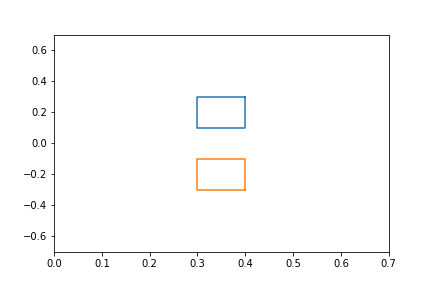
\includegraphics[width = \linewidth]{img/obstacles.png}
    \caption{Two-dimensional workspace with two obstacles}
    \label{fig:exampleWorkspace}
\end{figure}
Assume the shoulder of human arm is located at position $(0.7,0.0)$, and the robot starts at $(0.0,0.0)$. 
While the visually-impaired user in navigating freely, the system must throw an interruption command when there is a chance of collision between the human hand and an obstacle, or human arm and an obstacle. 

It would be unwise to throw an interruption only when a collision occurs, since the human may be moving very quickly and could hurt themselves. 
This means that the strategy will inevitably require some form of collision prediction. 
A simple solution to this was to apply a magnification transform on the obstacles in the workspace. 
This will throw a interruption before the arm or hand collides with the actual obstacles in the workspace. 

Using this strategy for collision detection is not optimal as it has many inherent flaws. 
For instance, in situations where there are tight spaces between obstacles, the collision detection will still throw interruptions even though no actual collision is taking place. 
Furthermore, with increased number of obstacles, this strategy significantly reduces the navigable area for the human arm. 

The experiment only tracks the motion of the human hand. 
With this information, a line segment is drawn from the predefined human shoulder location to the human hand (this method assumes that the human arm is unbending and a rigid body). 
If the segment intersects with any of the magnified obstacles in the workspace, it is taken that a collision has occurred and an interruption is thrown. 
This interruption is in the form of an auditory warning asking the human to stop their free-navigation. 
Once that is done, the human hand position and final goal position is passed to the motion planner.

\subsection{Human-Arm Conscious Motion Planner}
The goal of the motion planner is to assist the human arm in moving from a precarious position to a position closer to the goal while avoiding potential collisions with obstacles. 
First the workspace is sampled to form a navigable graph, then graph is traversed given the start and endpoint through an optimal strategy. 
Integrated into the traversal strategy is a novel cost function that evaluates if the chosen path results in collision of the human arm with obstacles. 

The assistive robot used in this experiment is a 7-DOF Sawyer robot. 
While sampling, it is important to consider if it is possible for the robot to orient itself in the sampled configuration. 
To simplify this process, first we sampled in the two-dimensional workspace and used the IK solver to determine if it is possible to orient the robot in that configuration. 
If that is not possible, a new point in the workspace and tested.  
Once the workspace is sampled, neighbours to the sampled points are determined based on the proximity (according to the euclidean distance) in both the configuration space and navigation space. 

One problem that we faced was that during sampling, there were a lot of cases when the robot could not be configured in the required orientation. 
Hence sampling of a singular point was repeated multiple times as the IK solver repeatedly threw errors. 

To navigate the graph, we use the A* algorithm for its heuristic. 
In addition to the algorithm, we added an additional cost function that evaluates if a transition to a neighbouring node is safe for the human. 
Consider two points in the graph as shown in Figure \ref{fig:humanArmConscious}. 
\begin{figure*}[htpb]
  \centering
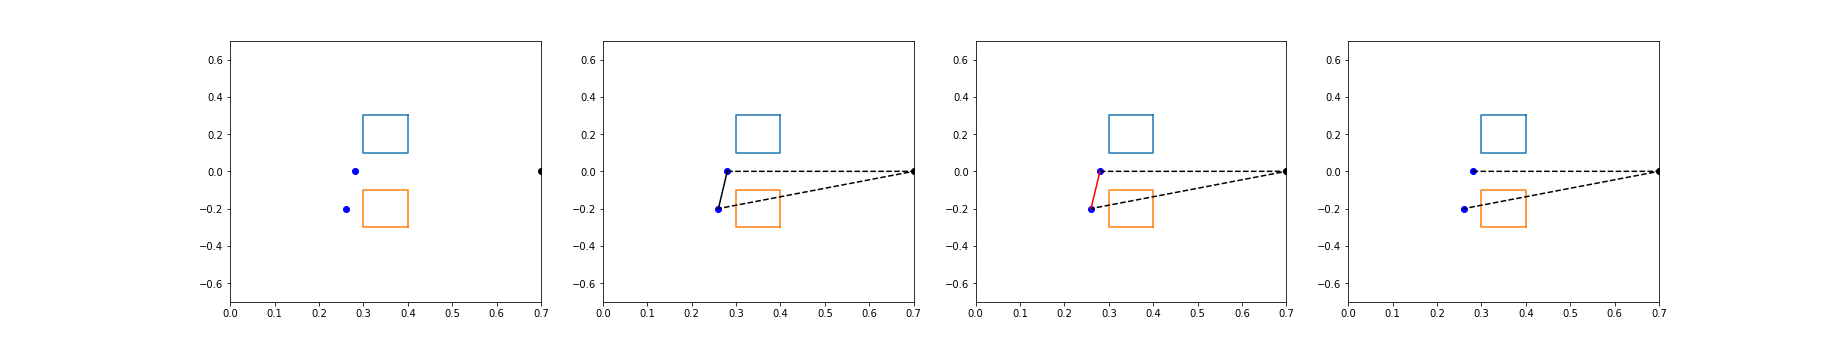
\includegraphics[width = \textwidth]{img/humanArmConscious.png}
  \caption{Human arm conscious cost function for motion planner}
  \label{fig:humanArmConscious}
\end{figure*}
We draw a polygon joining the two nodes and the human shoulder location. 
If the polygon intersects with any obstacles in the workspace, we increase the cost of transitioning between the node and its neighbour to infinity. 
This discourages the algorithm from following that transition. 

This additional cost function is rather basic and does not consider any additional properties such as arm comfort. 
It also does not take into consideration the fact that the human arm is a 2-DOF linkage that can offer greater maneuverability. 
However, it does take into consideration potential worst case scenarios and is guaranteed to provide safe trajectories. 

% Motionplanner: what is new in it? our contribution
% the platform we used and technical stuff (arm tracking method)


% Experimental design
\section{Experimental Design}
We are providing experimental design for in lab or in simulation environment. In simulation environment, we provide modified protocol to fit simulation environment. 

\subsection{In Lab procedure}
\begin{itemize}
    \item Human participants will be shown a 2D empty work space with the goal marked clearly. Once they have a general idea of work space, their hand will then be placed at the starting point, and then they will be blindfolded.
    \item Then work space will be populated with obstacles.
    \item The experiment will begin by asking the person to move their hand towards the goal while keeping it close to the work space surface.
    \item In the first run, the Sawyer manipulator will guide the human using the continuous kinesthetic guidance system.
    \item In the second run the human will be able to move freely through the work space, and the robot will provide an on-demand kinesthetic guidance system when needed. If the participant hand enters the collision zone, a technician would voice alert (indicated through the warning node) and the robot will guide the human out of the collision zone to a point in space where participant can continue to navigate to the goal.
\end{itemize}
\subsection{In Simulation Environment}
\begin{itemize}
    \item We expect humans to act accordingly in simulation. 
    \item Give a human arm coordinates near obstacles. 
    \item Feed it to the motion planner.
    \item Check what trajectory robot comes with to avoid the collision.
\end{itemize}

\subsection{Changes to System Components}
Due to the unforeseen campus closure, a lot of the technical components that were a part of this project (refer to Figure \ref{fig:TechnicalComponents}) could not be actualised. 
For instance, the `Hand tracker component', the `Workspace Map' and `Sawyer Manipulator' were either omitted, integrated into other components, or replaced with a simulated system.

Since we are no longer tracking a live human hand, the `Hand Tracker' component was omitted and instead the position was published manually. 
This is because we cannot test the algorithm's effectiveness in conjunction with a human, and instead are focusing only on the effectiveness of the motion planner. 
The `Workspace Map' was integrated into the motion planner and free-navigation interrupter, by hardcoding the obstacle positions and dimensions. 
This is since we are not using an RBG camera to monitor the workspace.  
The `Sawyer manipulator' was replaced with a Gazebo simulator. 
It does not have any function other than displaying the output from the motion planner.
\begin{figure}[H]
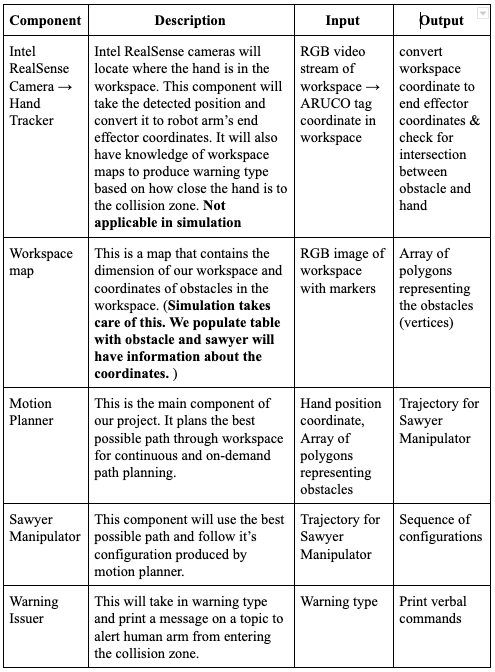
\includegraphics[width=\linewidth]{img/techcomponent.png}
\caption{Technical Components}
\label{fig:TechnicalComponents}
\end{figure}

% result
\section{Evaluation}
We measure result based on two metrics, objective and subjective metrics as shown in Figure \ref{fig:objectiveMetrics} and \ref{fig:subjectiveMetrics}. 
\begin{figure}
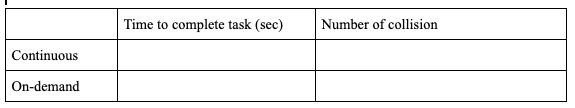
\includegraphics[width=8cm]{img/objectivemetrics.png}
\caption{Objective Metrics}
\label{fig:objectiveMetrics}
\end{figure}
\begin{figure}
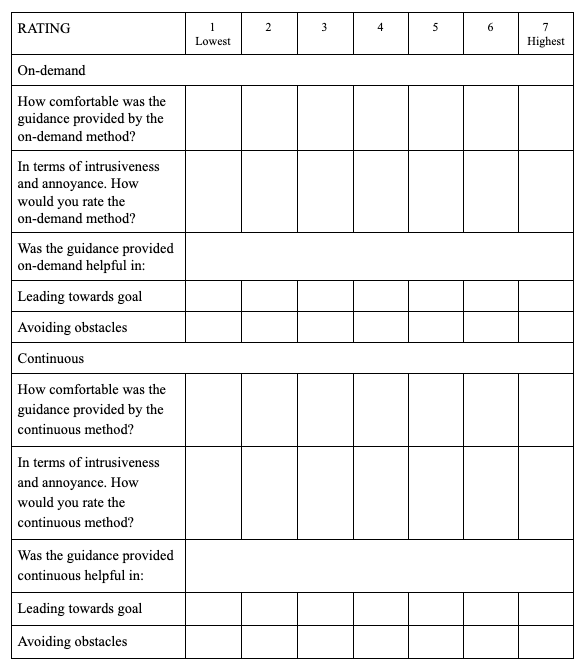
\includegraphics[width=8cm]{img/subjectivemetrics.png}
\caption{Subjective Metrics}
\label{fig:subjectiveMetrics}
\end{figure}
We were not able to get data for subjective metrics due to COVID-19. 
Furthermore, the extent to which we can gather objective data will also be limited. 
If and when we are able to perform the experiment in lab, one important factor to take into consideration is that the response of blindfolded people with perfect vision and people who are visually impaired might be different. 
People who are blindfolded might get more nervous or respond differently when navigating through the environment which might lead to bias is result. 
It would be preferable to test the algorithm with originally visually-impaired subjects. 
However in its current state, the algorithm is not complete and safe for implementation. 

Additionally, since the experiment is running in simulation, there are certain parameters that cannot be fully evaluated. 
For instance, it is not possible to measure the total duration of navigation with on-demand and continuous guidance, since we cannot account for the human arm travel duration in the former case. 
All that can be extracted from the simulation is duration to determine the motion plan. 
It is also not possible to determine if, even after determining the motion plan, there will be any collisions between obstacles and the human. 
% \setlength{\belowcaptionskip}
\begin{figure}
    \centering
    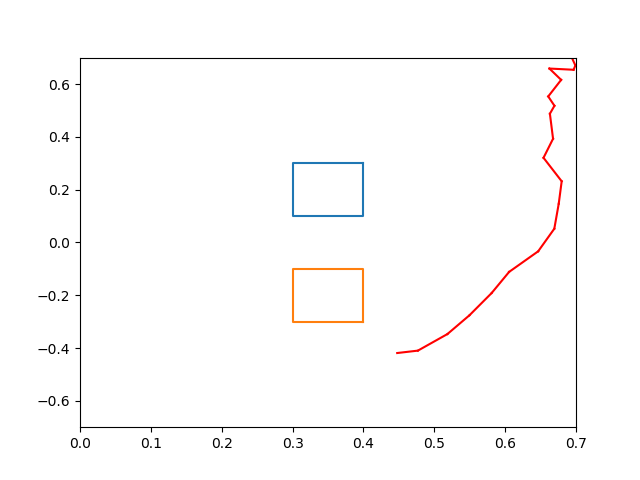
\includegraphics[width = \linewidth]{img/continuous_30s03ms.png}
    \caption{Trajectory for continuous guidance - duration 30s 3ms}
    \label{fig:ContinuousGuidance}
\end{figure}
\begin{figure}
    \centering
    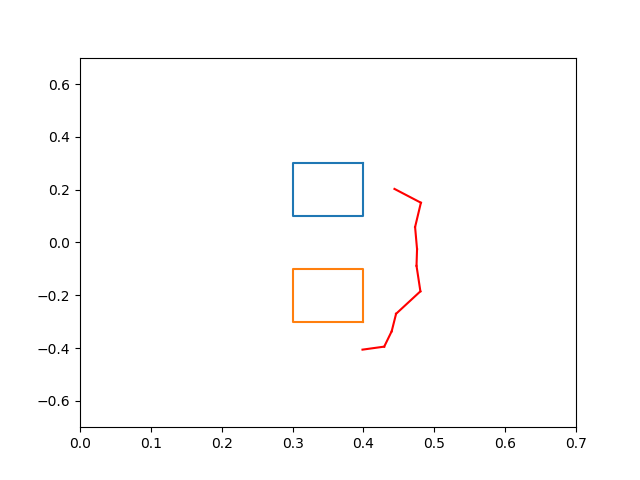
\includegraphics[width = \linewidth]{img/ondemand_18s03ms.png}
    \caption{Trajectory for on-demand guidance - duration 18s 4ms}
    \label{fig:OndemandGuidance}
\end{figure}
In the case of continuous and on-demand guidance, an example trajectory is shown in Figure \ref{fig:ContinuousGuidance} and \ref{fig:OndemandGuidance}. 
It is an obvious find that the continuous guidance motion plan had a longer duration as opposed to the on-demand plan, since the distance over which the trajectory is planned is longer. 
The duration for the motion plan with continuous guidance was 30s 3ms, and with on-demand guidance it was 18s 4ms. 
Note how the trajectory ensures that human arm does not collide with the obstacles in the workspace. 
However, also note that the issue which was brought up before about the stringency of the human arm conscious cost function is evident in the results. 
As the trajectory moves beyond the obstacles, the cost function, which does not consider the flexibility of the human arm, starts to limit exploration. 

Furthermore, because of the heuristic in the A* algorithm, the graph traversal is excessively greedy and can sometimes take a path towards the goal which results in a position that is disadvantageous for the human, although it is still closer to the goal. 
Possible methods to improve the strategy are discussed in the discussion section.  

% evaluation
\section{Discussion}
Due to unable to perform experiment with participants, it results in no data for subjective metrics, and insufficient or indescriptive data for the objective metrics. 
Without an experiment with live subjects we could not obtain sufficient data to derive a conclusion. 
Hence we were unable to properly evaluate our hypotheses. 
Although we were able to develop a motion planner that satisfies the requirements of the problem, we could not go beyond a superficial evaluation of its effectiveness. 
We also could not completely tailor the experiment such that it could be properly evaluated in a simulated environment. 
This was since the investigation was highly reliant on the human component, and their reliance on robot for guidance. 

One area for improvement with the motion planning algorithm would be to consider the human arm's ability to pivot at the elbow. 
If we consider this property, the stringency of the cost function can be reduced, which will allow the guidance to extend further. 
Furthermore, we also could improve the guidance strategy by implementing ways to incorporate audio cues and warnings. 
In this experiment, the audio interruptions were provided by the researchers. 
We also did not consider arm comfort in the motion plan. 
This is especially important when the human could use either their left or right arm. 
Depending on that, the human arm will have preferable configurations and range of motions that should be considered.

The investigation could be further improved by considering a three-dimensional workspace to make it more realistic and add to the complexity. 
In addition to this, we could also consider an improved method of sampling the workspace. 
The current strategy to randomly sample the workspace and find robot configuration through the IK solver was found to be inefficient, and it also resulted in blind spots in the workspace (as the robot could not configure itself to reach those regions). 

We are leaving subjective metrics as guideline for future work. 
In the future, we can take existing work that we have completed so far, and implement the experiment in the lab. 
We hope to improve the algorithm and finally test it with visually-impaired subjects to gain accurate primary data. 

%areas for improvement
%possible extensions to the project
% how can someone do this experiment in the future. 

% conclusion
\section{Conclusion}
%summary and reiterate hypothesis and if it was satisfied
Although we could not proof our hypothesis due to lack of experiment with participant, we completed the components that adds complexity to existing kinesthetic guidance. In this paper, we implemented two kinesthetic guidance methods, continuous and on-demand kinesthetic guidance and explained motion planner for both methods. We believe these methods will contributes towards future experiment. In the future, we can also explore preference between audio guidance and on-demand guidance to promote independence for people with visually impairment. 


\cite{FinalVideo}
% \textbf{Final video presentation link: \cite{FinalVideo}}



% \newpage\newpage


%%
%% The next two lines define the bibliography style to be used, and
%% the bibliography file.
\bibliographystyle{ieeetr}
\bibliography{ref}

%%
%% If your work has an appendix, this is the place to put it.
\appendix



\end{document}
\endinput
%%
%% End of file `sample-authordraft.tex'.
